\documentclass[]{article}

\usepackage{color}
\usepackage{graphicx}
\usepackage{amsmath}
\usepackage{amsfonts}
\usepackage{mathrsfs}
\usepackage[symbol]{footmisc}
\newcommand{\red}[1]{\textbf{\color{red} #1}}

\newcommand{\revision}[1]{\textbf{#1}}


% Derivatives and differentials
\newcommand{\ds}{~\text{d}\boldsymbol{s}}
\newcommand{\dzeta}{~\text{d}\boldsymbol{\zeta}}
\newcommand{\pder}[2]{\frac{\partial #1}{\partial #2}}
\newcommand{\bs}[1]{\boldsymbol{#1}}
\newcommand{\dx}{\text{d}\boldsymbol{x}}
\newcommand{\dt}{\text{d}t}
\newcommand{\ddt}[1]{\frac{\text{d} #1}{\text{d} t}}
% Integrals
\newcommand{\stint}{\int_{0}^{T} \int_{\Omega}}
\newcommand{\sint}{\int_{\Omega}}
\newcommand{\Tint}{\int_{0}^{T}}
\newcommand{\tint}{\int_{0}^{t}}
% Filtered variables
\newcommand{\utilde}{\widetilde{\bs{u}}}
\newcommand{\ptilde}{\widetilde{p}}
\newcommand{\ctnhat}[1]{\widehat{C}_{T,#1}'}
\newcommand{\ctihat}{\widehat{C}_{T,i}'}
\newcommand{\cthat}{\widehat{C}_T'}
% Other symbols
\newcommand{\ctmax}{C_{T,\text{max}}'}
\newcommand{\cti}{C_{T,i}'}
\newcommand{\ctn}[1]{C_{T,#1}'}
\newcommand{\R}{\mathscr{R}}
\newcommand{\J}{\mathscr{J}}
\newcommand{\Jtilde}{\tilde{\mathscr{J}}}
\newcommand{\Jgrad}{\nabla \Jtilde}
\newcommand{\Lagr}{\mathscr{L}}
\newcommand{\eperp}{\bs{e}_\perp}
\newcommand{\eperpi}{\bs{e}_{\perp,i}}
\newcommand{\etransi}{\bs{e}_{\parallel,i}}
\newcommand{\ex}{\bs{e}_x}
\newcommand{\ey}{\bs{e}_y}
\newcommand{\ez}{\bs{e}_z}
\newcommand{\eperpn}[1]{\bs{e}_{\perp,#1}}
\newcommand{\vi}{\frac{1}{A_i} \sint \R_i (\bs{s})~\utilde \cdot \eperpi \ds}
% Operators
\newcommand{\innerproduct}[2]{\bigg( #1, #2 \bigg)}
\newcommand{\innerproductsmall}[2]{\big( #1, #2 \big)}
\newcommand{\sumturbines}{\sum_{i=1}^{N_t}}
\newcommand{\diracdelta}{{\delta}}
\DeclareMathOperator*{\argmin}{arg\,min}




\usepackage[margin=1.5in]{geometry}

\setlength{\parindent}{0pt}
\setlength{\parskip}{0.5\baselineskip}

%opening
\title{Response to Reviewer 2}
\author{}
\date{}

\begin{document}

\maketitle

We are pleased with the positive assessment of our work by the reviewer and thank him/her for thoroughly reading our manuscript and for providing constructive input. The responses to the reviewer's comments and adaptations in the revised manuscript are discussed below.

\hrulefill

\paragraph{Reviewer} \textit{The paper presents very interesting research related to control of wind farms using yaw and induction control mechanism, as well as combination of both. Using large-eddy simulations (LES) combined with adjoint-based optimization the authors showed significant improvement in power generation for 4 $\times$ 4 wind farm layout. Both, uniform and turbulent inflow conditions were considered with 8 different control strategies for each case. The paper is well written and suggested for publication after addressing the following comments:}


\section*{Comments}
\hrulefill

\paragraph{1. Reviewer} \textit{The main novelty in current paper compared to Ref. [14] is the addition of the yawing. This should be clearly stated in the Introduction part, e.g. in the last paragraph (lines 107-118)}

\paragraph{Response} This is correct. We have made this more explicit in the revised manuscript in lines 107 -- 118 as follows: 

``
In the current manuscript, we aim to fill some of the aforementioned gaps in wind-farm control research \textbf{using the dynamic control approach based on large-eddy simulation and optimization as introduced by Goit \& Meyers [11]. The main novelty of the current work is the inclusion of yaw control, in addition to the induction control considered in previous studies [11, 12, 14].} Based on a demonstration $\dots$
''

\hrulefill

\paragraph{2. Reviewer} \textit{Line 137: "...in an accurate model with full state...", references should be provided here with previous studies using this model to show its accuracy. Authors already cited them in Introduction but it would be worth to repeat some of them here.}

\paragraph{Response} Done. References to previous studies using the same model were added (\red{line XX, p YY}):

``
... accurate model with full state information (see, e.g. Refs. [11--14]), i.e. using large-eddy simulation ...
''

\red{WM: Heb hier gereferereerd naar onze vorige optimal controls met LES studies... Weet niet of hij dit exact bedoelt, of eerder naar in welke mate LES geschikt is voor wind-farm simulaties (dit vermelden we niet echt in de introductie, dus ben niet zeker...) Evt. te bespreken. }

\hrulefill

\paragraph{3. Reviewer} \textit{Line 184: L-BFGS-B. It might be good to spell it out for clarity.}

\paragraph{Response} Done. We updated the revised manuscript as follows (\red{line XX, p. YY}):

`` 
$\dots$ solved using the \revision{L-BFGS-B (limited-memory Broyden--Fletcher--Goldfarb--Shanno with bounds support) algorithm [40]}, which is an $\dots$
''

\hrulefill

\paragraph{4. Reviewer} \textit{Line 202-203 should be placed before Eq. 13.}

\paragraph{Response} Done.

\hrulefill

\paragraph{5. Reviewer} \textit{Line 211: corresponding notation for dimensions should be provided, or reference to Table 1 should be given right after 4.8x2.4x1}

\paragraph{Response} Done. In addition, we changed the notation of the domain height from $H$ to $L_z$ for consistency. The manuscript is revised as follows (\red{line XX, p. YY}):

`` 
$\dots$ has a \revision{total dimension of $L_x \times L_y \times L_z = 4.8 \times 2.4 \times 1 $ km$^3$, with $L_x, L_y$, and $L_z$ the streamwise, transversal, and vertical extent of the domain respectively. This domain is discretized on a grid of $N_x \times N_y \times N_z = 256 \times 128 \times 128$ gridpoints.} The final $\dots$
''

\hrulefill

\paragraph{6. Reviewer} \textit{Line 217: Define Zh}

\paragraph{Response} Done. The manuscript is updated as follows:

``
$\dots$, \revision{and the vertical location of the turbine hubs $z_h$ is placed at the vertical mid-plane of the domain, i.e. $z_h/L_z = 0.5$,} in order to minimize $\dots$
''

\hrulefill

\paragraph{7. Reviewer} \textit{Line 215-218: Figure should be provided with 3D domain, to clarify the vertical placement of the turbine.}

\paragraph{Response} Done, Figure 3 has been updated in the revised manuscript, and is shown above.

\begin{figure}
	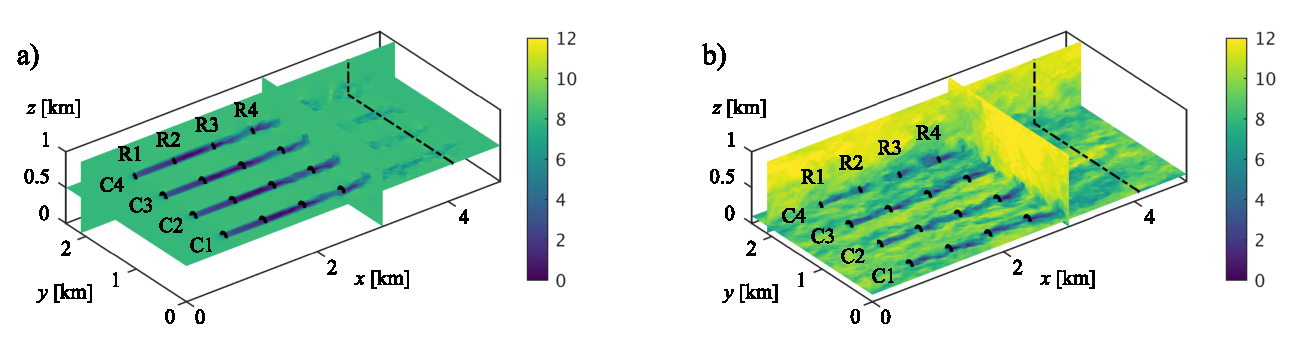
\includegraphics[width=\textwidth]{figure3_revised}
\end{figure}



\hrulefill

\paragraph{8. Reviewer} \textit{It might be good to provide brief comments on sensitivity of the solution to control time or explain the choice of current control time. If it was done previously, reference would be enough.}

\paragraph{Response} This is a valid comment. We have updated the discussion in the manuscript where time horizons $T$ and $T_A$ are selected as follows (\red{Section 3.1, line XX p YY}):

``
\revision{Within the context of the receding-horizon methodology introduced in Section 2, the optimization is performed over discrete time windows with optimization horizon $T$ and flow advancement time $T_A$. Ideally, one would take a very large optimization horizon $T$, and a small flow advancement time $T_A$ before recomputing the optimal control problem. However, in practice, $T$ is limited due to the inherent chaotic nature of turbulent flows that complicates control over long time horizons, and $T_A$ should not be taken too small to avoid excessive computational costs. In the current work, we use 6 consecutive windows, each with an optimization horizon $T=300$~s and a flow advancement time of $T_A = T/2= 150$~s, resulting in a total control time of 900~s. Note that, given a wind-farm length of $3 \times 6D = 1 800$ m and a free-stream velocity $U_\infty = 8$ m s$^{-1}$, the wind-farm flowthrough time is approximately 225 s. Hence, the total control time comprises about 4 flowthroughs, and the optimization horizon within each window covers about 1.33 flowthrough times. Because of the latter, each turbine row has the opportunity to take into account interaction with every downstream row, and the sensitivity of power gains to the optimization horizon $T$ is expected to be limited.} All time-averaged results ...
''

Furthermore, we quantified the sensitivity of attainable power gains to $T/T_A$ in previous work, and mention this explicitly in the revised manuscript (\red{Section 3.1, line XX p YY}):
`` 
... or all turbines. \revision{The sensitivity of attainable power gains to $T/T_A$, initial control guesses, and optimizer settings has been shown to be limited in a prior study [14].} Simulation and optimization parameters ...
''

\hrulefill

\paragraph{9. Reviewer} \textit{It looks like no towers were included in current simulation. The authors should clearly state it in Introduction and provide comments on importance/non-importance of tower inclusion in Summary part. It could be provided after the authors provided comments on the effect of stratification.}

\paragraph{Response} Indeed, the turbines are modeled without adding a turbine tower. We mention this explicitly in the revised manuscript as (Section 2, \red{line XX, p YY}):

``
... non-rotating actuator disk model (see, e.g., Ref [38]). \revision{Turbine towers are not included.} For each ...
''

Prior studies in literature have shown that including towers and nacelles in wind-farm LES can improve the near-wake characteristics, although we expect that, at the grid resolution of the current paper, the improvement would be relatively small. However, we agree that in the future this would be a valuable improvement to the fidelity of the turbine model. Moreover, when considering loads as indicated in the future work section, assessment of tower loading is of high importance. As suggested by the reviewer, we include this in the Conclusions section as follows:

``
\revision{The current optimization studies have been performed using relatively simple non-rotating actuator disk models for the wind turbine rotors without the inclusion of towers or nacelles. Although it has been shown that, by using this approach, the fidelity of far wake characteristics is satisfactory, the credibility of the current power gains and control strategies in practice could be further increased through wind-tunnel testing and similar optimization studies with more detailed turbine models, e.g. by adding drag forces for the tower and nacelle or by representing the rotor with an actuator line model. These are left for future work.} Finally, note that the current study optimizes power at all costs, and did not account for any undesirable loading characteristics. These should also be considered upon thoroughly comparing induction and yaw control for practical purposes. \revision{In this latter case, a detailed turbine representation is of high importance.}
''

\hrulefill

\paragraph{10. Reviewer} \textit{In Table 1: the expression for precursor pressure gradient is inconsistent with the one defined in line 220, i.e. rho is missing.}

\paragraph{Response} Thanks for pointing this out. Fixed. 

\hrulefill

\paragraph{11. Reviewer} \textit{Line 335: The authors clearly stated that the optimal control is heterogeneous, however no comments on why it is heterogeneous were provided. It was stated that turbine can pick either wake meandering type of motion or wake redirection, however what will determine this decision?}

\paragraph{Response} As mentioned in the manuscript, the flow conditions of the different columns are equivalent in a \emph{statistical} sense. However, the gradient, and hence the updates to optimized control iterates, are based on \emph{instantaneous} flow conditions. Small instantaneous differences in flow conditions between different columns can hence tip the balance between different flow control mechanisms suchs as wake meandering, wake redirection through clockwise yawing, or wake redirection through counterclockwise yawing. Which mechanism is chosen depends on the initial steps in the optimization process when the optimizer is settling into a local optimum of the cost functional landscape. These steps are based on the gradient, which is found by solving the turbulent adjoint equations. Therefore, it is not possible to determine \emph{a priori} which method will be chosen by the optimizer. The fact that, after some time, all turbines seem to abandon the meandering mechanism in favor of the redirection mechanism seems to indicate that a global optimization approach would probably always yield the wake redirection mechanism.

We included the reason for different mechanisms in the optimized controls as follows (Section 4.2.2, \red{line XX, p YY}):
``
... their behavior in an optimal control setting is heterogeneous. \revision{The reason for this is that the cost functional gradient used in the optimization process is based on the instantaneous flow conditions through the adjoint equations. These conditions are not the same for different columns, e.g. the turbulence in the wakes behind the third row observed in Figure 5 is different for every column, which can cause the optimizer to converge to a different dominant control mechanism in different columns.} For example, ...
''

\hrulefill

\paragraph{12. Reviewer} \textit{Figure 5: The blue color for C4 and green color for C2 very hard to see, especially on I3Y case.}

\paragraph{Response} Thank your for this justified comment. We have plotted all turbine locations in black in the revised version of Figure 5 (and the corresponding Figure 11 for turbulent inflow).

\hrulefill

\paragraph{13. Reviewer} \textit{Figure 6 shows that for uniform inflow in a reference case the turbine in a second row will be producing almost 90\% less power then upstream. As a reader I would be interested to see previous studies on this. Adding corresponding references would be enough.}

\paragraph{Response} Indeed, power losses in uniform inflow conditions can be very large due to artificially stabilized wakes. In the submitted manuscript, we already mentioned that such conditions are somewhat artificial. We have expanded this discussion with some references in the revised manuscript. Furthermore, we added some references that also quantify severe losses under uniform inflow. A direct comparison between our results and prior work is not possible due to the dependence on numerical solver details, as indicated in the revised manuscript. The manuscript has been updated as follows (Section 3.1 \red{line XX, p YY}):

``
... These flow conditions can be regarded as somewhat artificial since, in the atmospheric boundary layer, background turbulence typically causes instant wake transition behind the turbine rotor. \revision{Furthermore, it is documented in literature that numerical details such as grid resolution, subgrid-scale modeling, and turbine models can have a significant impact on simulation results , whereas in turbulent inflow this is much less the case  [49-51]. In practice, this tends to lead to artificially stabilized wakes with very low farm efficiencies (see, e.g., Refs [52,53]).} Nevertheless, ...
''


Also, when discussing the power extraction of the refernece case in uniform inflow, we refer to this discussion (Section 4.2.1 \red{line XX, p YY}):
``
 As expected \revision{from the discussion in Section 3.1}, the efficiency of the uncontrolled reference farm R is very low at around $40\%$. ...
''

\hrulefill

\paragraph{14. Reviewer} \textit{Figure 7: Add tick labels to X-axis, i.e. to Time. (Same for Fig. 13)}

\paragraph{Response} We thank the reviewer for pointing out the missing labels, this has been corrected in the revised versions of Figures 7 and 13. Note that, in response to comments from another reviewer, we have reduced the amount of information in these figures somewhat for better clarity. 

\hrulefill

\paragraph{15. Reviewer} \textit{Line 424: "...steady uniform inflow cases", would it be better to use word "constant uniform inflow cases", to avoid any confusion with steady-state analysis.}

\paragraph{Response} We have updated the manuscript to consistently use the word 'constant' instead of 'steady' when mentioning the inflow conditions. (see revised manuscript)

\hrulefill

\paragraph{16. Reviewer} \textit{Line 596: the "and" is missing in "... yaw angle equation \_\_\_ the adjoint gradient"}

\paragraph{Response} Thanks for pointing this out. Fixed.

\hrulefill

\paragraph{17. Reviewer} \textit{In Eq. A13 $\rho_i$, $\gamma_i$ and $\chi_i$ should be defined. Currently they are defined in A.4.}

\paragraph{Response} Thanks for pointing this out. The manuscript has been updated as follows (\red{line XX, p YY}):

``
adjoint variables \revision{$\bs{q}^* = [\bs{\xi}, \pi, \sigma_1, \dots, \sigma_{N_t}, \eta_1, \dots, \eta_{N_t}, \rho_1, \dots, \rho_{N_t}, \bs{\gamma_1}, \dots, \bs{\gamma}_{N_t}, \chi_1, \dots \chi_{N_t}]$, which serve as Lagrange multipliers. The additional variables $\rho_i, \bs{\gamma}_i$, and $\chi_i$ are the adjoint counterparts of $\R_i, \eperpi$, and $V_i$, resulting from including the definitions of the latter as explicit constraints in (A10 - A12). The resulting Lagrangian is expressed as follows:}
''

\hrulefill

\end{document}
